\section{Naively Looking at the Poset Structure}
\label{tree:xy:grid}

In the previous section, we have shown how one could derive a poset structure
from the \XY set. We also saw that one can sort this \XY poset with
merging algorithm of \Cref{tree:merging:kgeq3}
using at most \(n^2 \log n + \BigO{n}\) comparisons. Indeed, what we
did in this section was modeling the Sorting \XY problem as the problem of
Sorting under Partial Information. We then solved the problem with a
straightforward algorithm.

In \Cref{tree:supi}, we have seen that there are algorithms solving the \SUPI
problem in \BigO{\log e(\P)} comparisons. We wonder if it is possible to prove
that, if we are only allowed to exploit the grid structure of the \XY poset,
then Sorting \XY cannot be solved in less than \(n^2 \log n + \BigO{n}\)
comparisons. In other words, we want to prove that the approach taken in the
previous section is optimal up to a linear term.

We already saw that the Hasse diagram of the poset \XY can be drawn as a grid.
This grid is finite and has a \(\hat{0}\) and a \(\hat{1}\). Moreover, any
two elements of this grid have a unique infimum and supremum. When this three
conditions are met for a poset, we call this poset a bounded lattice. We say
that the poset \XY is a \( n \times n \) bounded lattice.

We show that
\begin{theorem}[Number of linear extensions of the \( n \times n \) lattice]
Given a \( n \times n \) lattice \(\P\),
\begin{displaymath}
e(\P) = \frac{n^2!}{\prod_{k=1}^{2n-1} k^{n - \abs{n-k}}}.
\end{displaymath}
\end{theorem}
Note that an alternative way of writing \(e(\P)\) is
\begin{displaymath}
e(\P) = n^2! \cdot \mleft(\prod_{k=1}^{n-1} k!\mright)^2 \cdot
\mleft(\prod_{k=1}^{2n-1} k!\mright)^{-1}.
\end{displaymath}

To prove this theorem, we introduce the notion of Ferrers diagrams and standard Young tableaux.

A \emph{Ferrers diagram} can be seen as a set of square tiles arranged in a
rectangular
box divided in rows and columns. They are arranged so that there cannot be any space between two tiles
lying on the same row or column and there can never be a row that contains more
tiles than another row above it. Moreover, there cannot be space left between
the left side of the box and the first tile of each row. An example of a
Ferrers diagram is given in \ref{fig:xy:lattice:ferrers}.

A \emph{Young tableau} is a special way of labelling the \(n\) tiles of a Ferrers
diagram. If a Ferrers diagram is made of $n$ tiles, then a Young tableau drawn
on this diagram labels its tiles with the numbers from $1$ to $n$. We call
\emph{standard} a Young tableau having the following property:
if one reads tile labels of rows (from left to right) or
columns (from top to bottom) of this tableau, one should only encounter increasing sequences of
numbers. An example of a standard Young tableau is given in
\ref{fig:xy:lattice:young}.

\begin{figure}
\centering
\begin{subfigure}[t]{0.47\textwidth}
\centering
	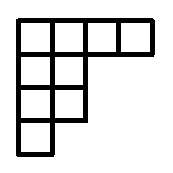
\includegraphics[width=0.4\textwidth]{fig/x+y/lattice/ferrers}
	\subcaption{Example of a Ferrers diagram with $9$ tiles. The shape of this
diagram is \(\lambda = (4,2,2,1)\).}
	\label{fig:xy:lattice:ferrers}
\end{subfigure}
~
\begin{subfigure}[t]{0.47\textwidth}
\centering
	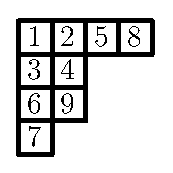
\includegraphics[width=0.4\textwidth]{fig/x+y/lattice/young}
	\subcaption{Example of a standard Young tableau in the Ferrers diagram of
\ref{fig:xy:lattice:ferrers}.}
	\label{fig:xy:lattice:young}
\end{subfigure}
\caption{Ferrers diagrams and Young tableaux.}
\end{figure}

The number of standard Young tableaux for a given Ferrers diagram shape
\(\lambda\) can be computed using the hook-length formula \(d_{\lambda}\).
\begin{theorem}[\citet*{frame:1954}]
\label{theorem:xy:lattice:hook}
Let \(\lambda = (\lambda_1,\ldots,\lambda_m)\) be a partition of the natural
number \(n\), \ie such that \(\sum_i \lambda_i = n\). The number of standard
Young tableaux of shape \(\lambda\) is
\begin{displaymath}
d_{\lambda} = \frac{n!}{\prod_{(i,j) \in \lambda} h_{\lambda}(i,j)}
\end{displaymath}
\end{theorem}

\(h_{\lambda}(i,j)\) denotes the length of an imaginary hook bending at
\((i,j)\). The \emph{hook} \(H_{\lambda}(i,j)\) is a subset of the tiles of
\(\lambda\) containing all tiles \((a,b)\) such that \(a = i\) and \(b \ge j\)
or \(b = j\) and \(a \ge i\). \ref{fig:xy:lattice:hooks} shows the hook length
at each tile and highlights the hook bending at \((2,1)\).

\begin{figure}
\centering
\begin{subfigure}[t]{0.47\textwidth}
\centering
	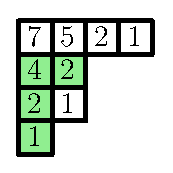
\includegraphics[width=0.4\textwidth]{fig/x+y/lattice/hooks}
	\subcaption{Ferrers diagram with hook length for each tile. The highlighted
region is the hook bending at \((2,1)\).}
	\label{fig:xy:lattice:hooks}
\end{subfigure}
~
\begin{subfigure}[t]{0.47\textwidth}
\centering
	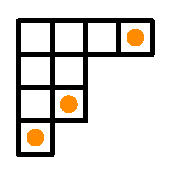
\includegraphics[width=0.4\textwidth]{fig/x+y/lattice/corners}
	\subcaption{Ferrers diagram with corners highlighted.}
	\label{fig:xy:lattice:corners}
\end{subfigure}
\caption{Hooks and corners in Ferrers diagrams.}
\end{figure}

The hook-length formula\footnote{
As a side note, the hook-length formula is closely related to
multidimensional Catalan numbers. The hook-length formula generates the numbers
on the diagonal of the matrix containing the \(\nth{n}\) \(m\)-dimensional
Catalan number at position \((m,n)\) \cite{OEIS:A060854}. The \(\nth{n}\)
\(m\)-dimensional Catalan numbers gives the number of shortest paths in the
\(m\)-dimensional unit grid from \( (0,\ldots,0) \) to \( (n,\ldots,n) \) such
that if \( (x_1,\ldots,x_m) \) is on a path then \( x_1 \le \cdots \le x_m\).
}
is attributed to \citet*{frame:1954}. Multiple ways to
prove \ref{theorem:xy:lattice:hook} are available in the literature. For more
information, one could start with \citet*{greene:1979} which gives a nice
probabilistic proof and pointers for further reading.

We give some insight into the proof given by \citet*{greene:1979}.
\ref{fig:xy:lattice:corners} highlights \emph{corners} of a Ferrers diagram. A
standard Young
tableau drawn in this diagram can only have its largest label given to
one of these corner tiles, otherwise we would obtain a row or a column that is
not increasing. The number of ways of arranging the standard Young tableau in the
Ferrers diagram of shape \(\lambda\) is thus the sum of possible tableaux of
size \(n-1\) over all shapes \(\lambda \setminus \gamma\) where the largest
label of our tableau of size \(n\) was given to corner \(\gamma\) of
\(\lambda\). Hence, the recurrence
\begin{equation}\label{equation:xy:lattice:reccurence}
d_{\lambda} = \sum_{\gamma \text{ is a corner of } \lambda} d_{\lambda
\setminus \gamma}
\end{equation}
holds. We can rewrite \ref{equation:xy:lattice:reccurence} as

\begin{equation}\label{equation:xy:lattice:walk}
\sum_{\gamma \text{ is a corner of } \lambda} \frac{d_{\lambda
\setminus \gamma}}{d_{\lambda}} = 1
\end{equation}

\citet*{greene:1979} define a hook walk to be a random walk starting at
any tile in the Ferrers diagram such that at each step, one moves uniformly at
random to another tile of the hook bending at the current tile.
They show that each term of the sum in \ref{equation:xy:lattice:walk} is
the probability for a single hook walk to end in each of the corners, proving
the theorem.

We return to our original problem. A \( n \times n \) bounded lattice can be regarded as a \( n \times n \)
standard Young tableau, \ie a standard Young tableau of shape
\( \lambda = \enum{ \lambda_1 , \ldots , \lambda_n } \)
with
\( \lambda_i = n, \Forall i \in \enum{1, \ldots, n}\).
\ref{fig:xy:lattice:xyhooks} shows the hook lengths
for the \( n \times n \) lattice, and thus for the \XY poset.
\begin{figure}
\centering
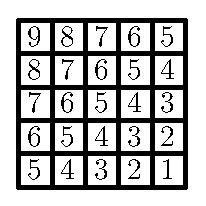
\includegraphics[width=0.24\textwidth]{fig/x+y/lattice/xyhooks}
\caption{Hook lengths for the \( n \times n \) lattice.}
\label{fig:xy:lattice:xyhooks}
\end{figure}
We need to show that counting tableaux is the same as counting linear
extensions. We label all \( n^2 \) nodes of \(\P\), the Hasse diagram of
\XY, with distinct etiquettes \(1,\ldots,n^2\). Suppose that we are
given a unique linear extension of \(\P\) that can be represented as a tuple
\( \omega = ( j_1 , \ldots , j_{n^2}) \)
with all \( j_i \) distinct and between \(1\) and \( n^2 \) using our
etiquettes. If we are given \( n^2 \) distinct numbers \( x_1,\ldots,x_{n^2} \)
then, according to our proof, there are \( d_{\lambda} \) ways to
fill our tableau with those numbers and to each filled tableau corresponds a
unique linear extension designated by \(\omega\). Hence,
\begin{displaymath}
e(\P) = d_{\lambda}.
\end{displaymath}

We prove that
\begin{theorem}[\ITLB for the problem of sorting a \(n \times n\) lattice]
Given a \( n \times n \) lattice \(\P\),
\begin{displaymath}
\log e(\P) = \BigOmega{n^2 \log n}
\end{displaymath}
\end{theorem}
\begin{proof}
Using Stirling's approximation,
\begin{align*}
e(\P) &= \frac{(n^2)!}{1 \cdot 2 \cdot 2 \cdot \cdots \cdot (2n-2) \cdot (2n-2) \cdot (2n-1)}\\
e(\P) &\ge \frac{(n^2)!}{(2n)^{n^2}}\\
\ln e(\P) &\ge \ln \group{\frac{(n^2)!}{(2n)^{n^2}}}\\
\lim_{n \to \infty} \ln e(\P) &\ge \ln{\group{\sqrt{2 \pi n^2}
\group{\frac{n^2}{\euler}}^{n^2}}}  - n^2 \ln n - n^2 \ln 2\\
\lim_{n \to \infty} \ln e(\P) &\ge \ln{\sqrt{2\pi}} + \ln n - n^2 \ln e + 2 n^2
\ln n - n^2 \ln n - n^2 \ln 2\\
\lim_{n \to \infty} \ln e(\P) &\ge n^2 \ln n - n^2 \ln (2\euler) + \ln n + \ln \sqrt{2\pi}\qedhere
\end{align*}
\end{proof}

Thus, solving \XY in \SmallO{n^2 \log n} comparisons is not possible if we only
consider the information contained in the poset structure. Moreover, to sort a
poset having the same structure, the merging technique explained earlier is
optimal. In \Cref{tree:xy:counting} we show that there is indeed more
information available.
